

\section{Benchmark Problems}

In this section we will test the performance of our designed algorithm (path representation) using some larger benchmark problems. Again we tested the parameter values in table \ref{table:question_3}. And we came to the conclusion that the optimal parameter values found in table \ref{table:question_3} are also the optimal parameter values for larger benchmark problems. We executed the tests on the benchmark problem containing 380 cities (\texttt{bcl380.tsp}). It is certainly not that logical that the parameter values that are optimal for small size problems are also the optimal values for larger size problems. Now that we have found the optimal parameter settings for our genetic algorithm, we can use the algorithm to solve some large benchmark problems.
In figure \ref{fig:belgium_tour_4} you can see the results for the Belgium tour benchmark problem. It seems that the GA found the optimal solution very quickly. We also did some experiments with two other benchmark problems. The results are shown in the figures \ref{fig:cities380_4_path}, \ref{fig:cities380_4_gen}, \ref{fig:benchmark_131_path} and \ref{fig:benchmark_131_gen}.

%\begin{figure}[!ht]
%  \centering
%    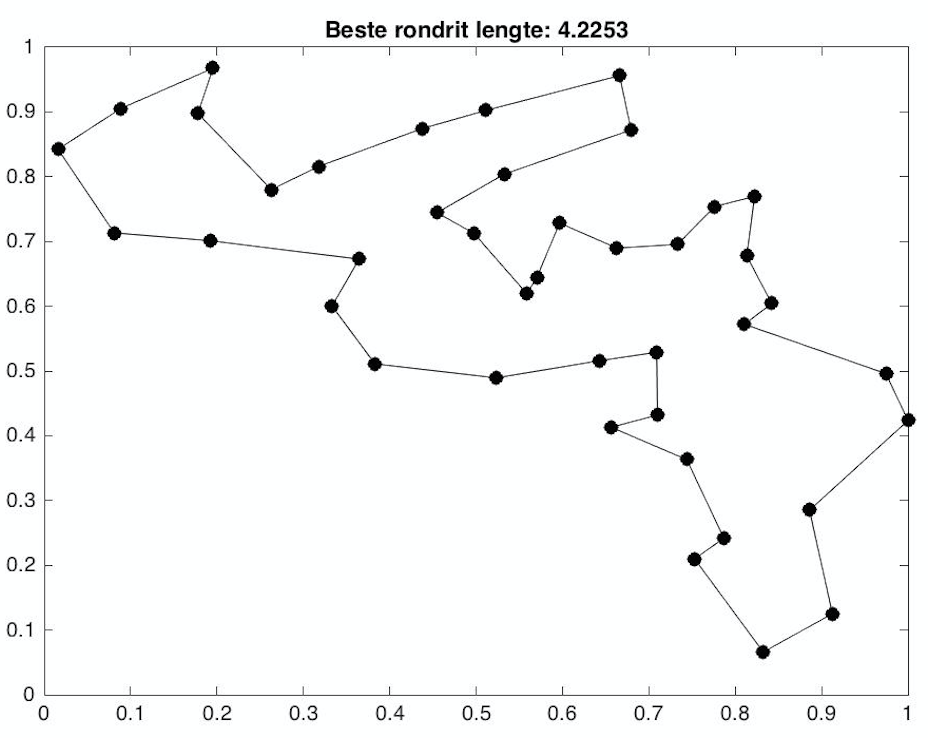
\includegraphics[width=0.5\textwidth]{../figures/figures_question_4/belgium_tour_path}
%      \caption{ There are }
%      \label{fig:belgium_path_4}
%\end{figure}

\begin{figure}[!]
\centering
\begin{subfigure}{.5\textwidth}
  \centering
  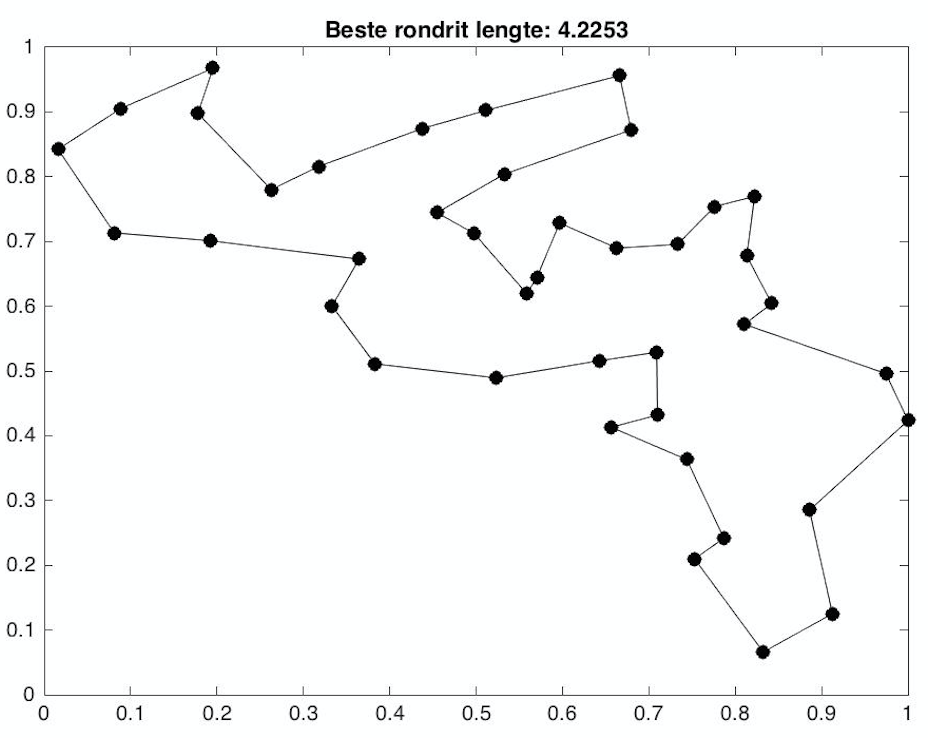
\includegraphics[width=.88\linewidth]{../figures/figures_question_4/belgium_tour_path}
  \caption{The most optimal tour found for the TSP problem. The distance of the tour is $4.2253$.\\ \ \\}
  \label{fig:belgium_tour_4_path}
\end{subfigure}%
\begin{subfigure}{.5\textwidth}
  \centering
  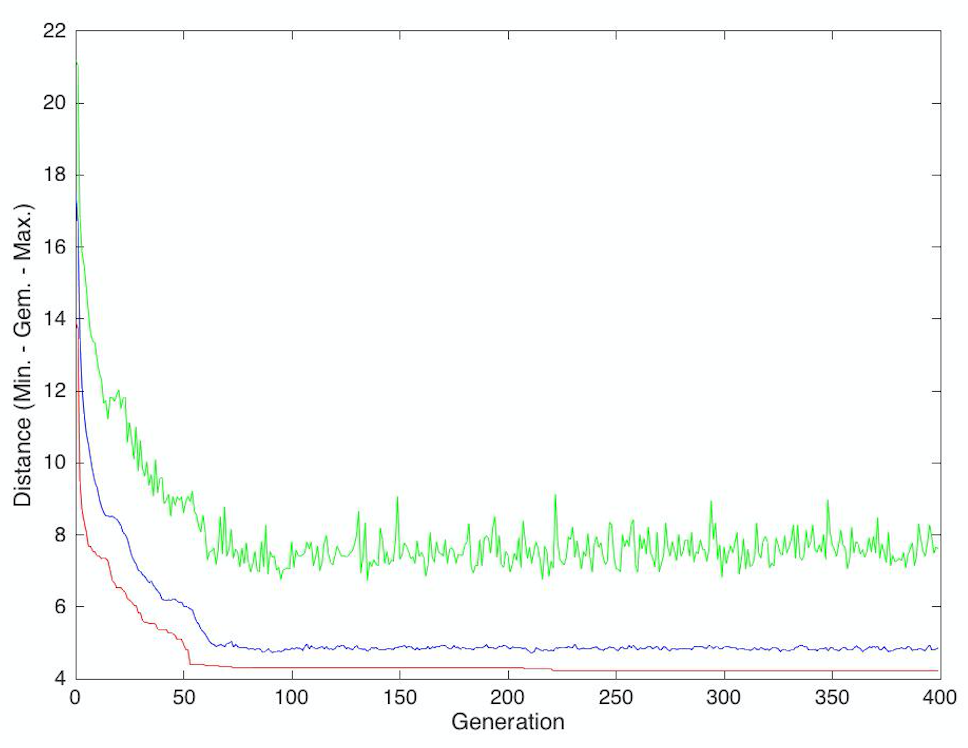
\includegraphics[width=.9\linewidth]{../figures/figures_question_4/belgium_tour_gen}
  \caption{The fitness values (tour distances) for the best(red), average(blue) and worst(green) candidate solution in every generation. \\}
  \label{fig:belgium_tour_4_gen}
\end{subfigure}
\caption{The benchmark TSP problem \texttt{belgiumtour.tsp} with 41 cities is solved here with path representation, order crossover and inversion mutation. The settings of the GA were \#IND = 400, \#GEN = 400, PR. MUT = $8\%$, PR. CROS = $80\%$, , ELITE = $15\%$, LP DET = ON.}
\label{fig:belgium_tour_4}
\end{figure}

\begin{figure}[!]
  \centering
    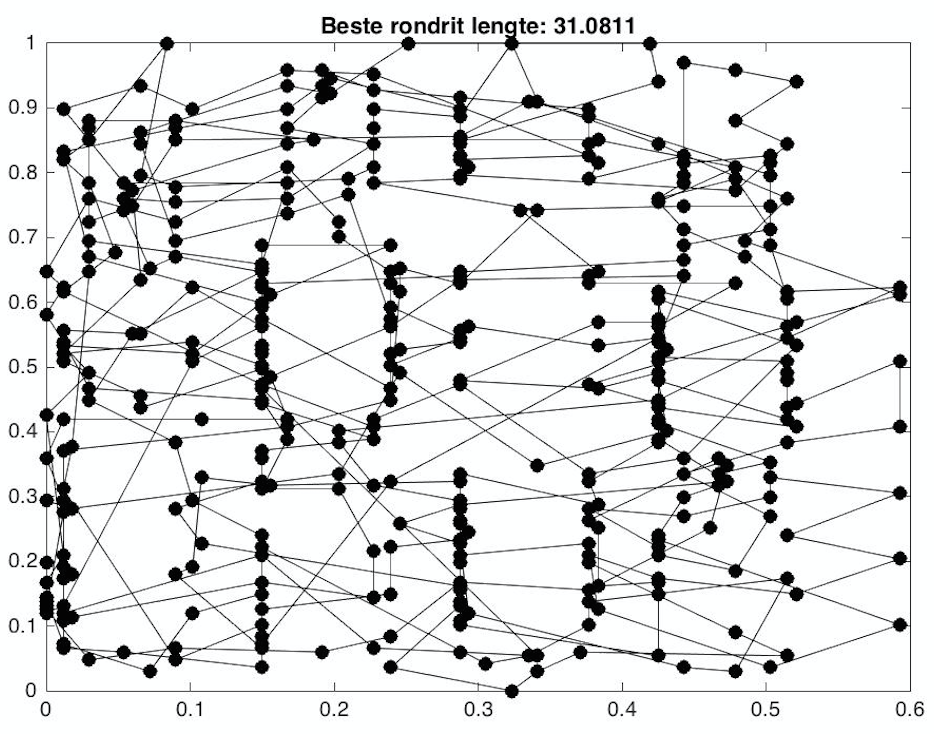
\includegraphics[width=0.7\textwidth]{../figures/figures_question_4/cities380_4_path}
      \caption{The benchmark TSP problem \texttt{belgiumtour.tsp} with 380 cities is solved here with path representation, order crossover and inversion mutation. The optimal candidate solution is far away from the best solution. The settings of the GA were \#IND = 500, \#GEN = 500, PR. MUT = $8\%$, PR. CROS = $80\%$ , ELITE = $15\%$, LP DET = ON. The CPU time needed was 440 seconds.}
      \label{fig:cities380_4_path}
\end{figure}

\begin{figure}[!]
  \centering
    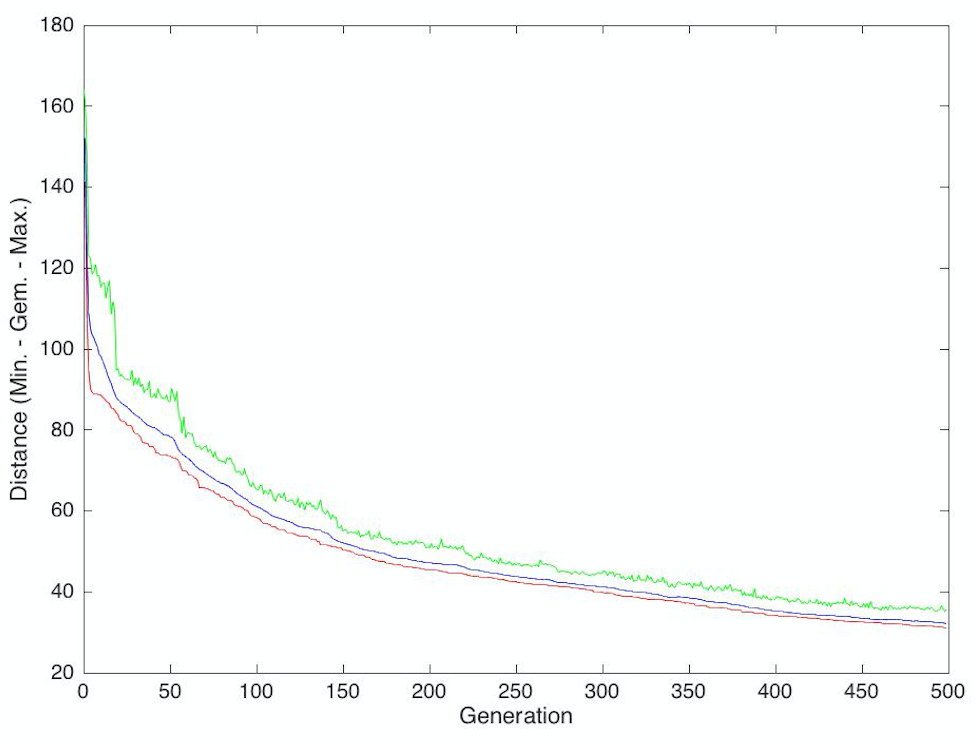
\includegraphics[width=0.7\textwidth]{../figures/figures_question_4/cities380_4_gen}
      \caption{The fitness values (tour distances) for the best(red), average(blue) and worst(green) candidate solution in every generation. This figure corresponds to the problem solved in figure \ref{fig:cities380_4_path}}
      \label{fig:cities380_4_gen}
\end{figure}

\begin{figure}[!]
  \centering
    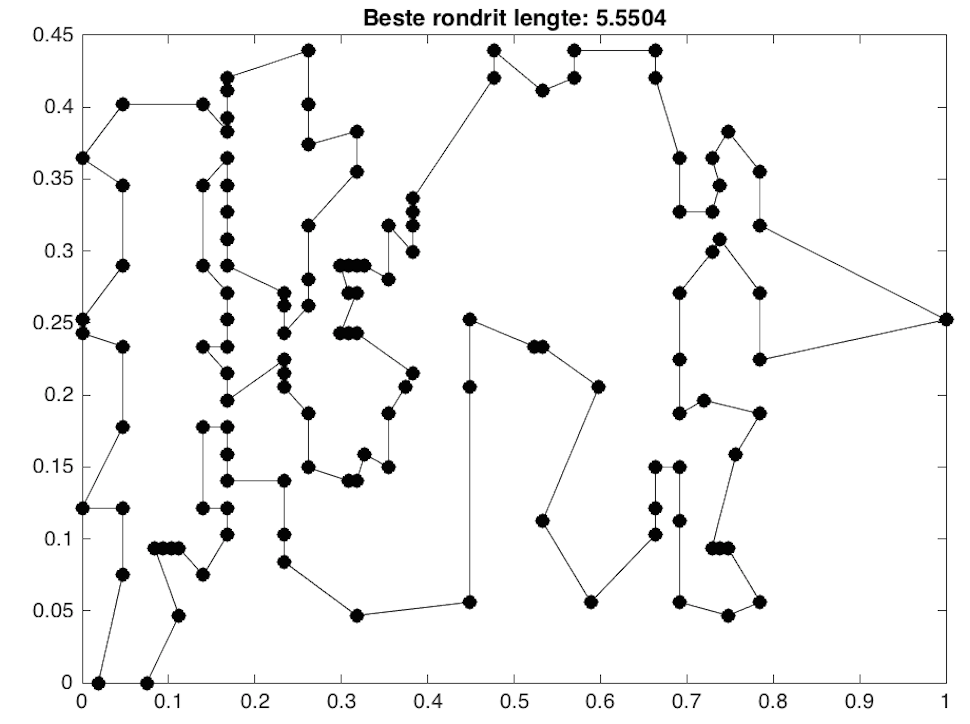
\includegraphics[width=0.7\textwidth]{../figures/figures_question_4/benchmark_131_path}
      \caption{The benchmark TSP problem \texttt{xqf131.tsp} with 131 cities is solved here with path representation, order crossover and inversion mutation. The optimal candidate solution is very good. The settings of the GA were \#IND = 1000, \#GEN = 1000, PR. MUT = $8\%$, PR. CROS = $80\%$ , ELITE = $15\%$, LP DET = ON. The CPU time needed was 584 seconds.}
      \label{fig:benchmark_131_path}
\end{figure}

\begin{figure}[!]
  \centering
    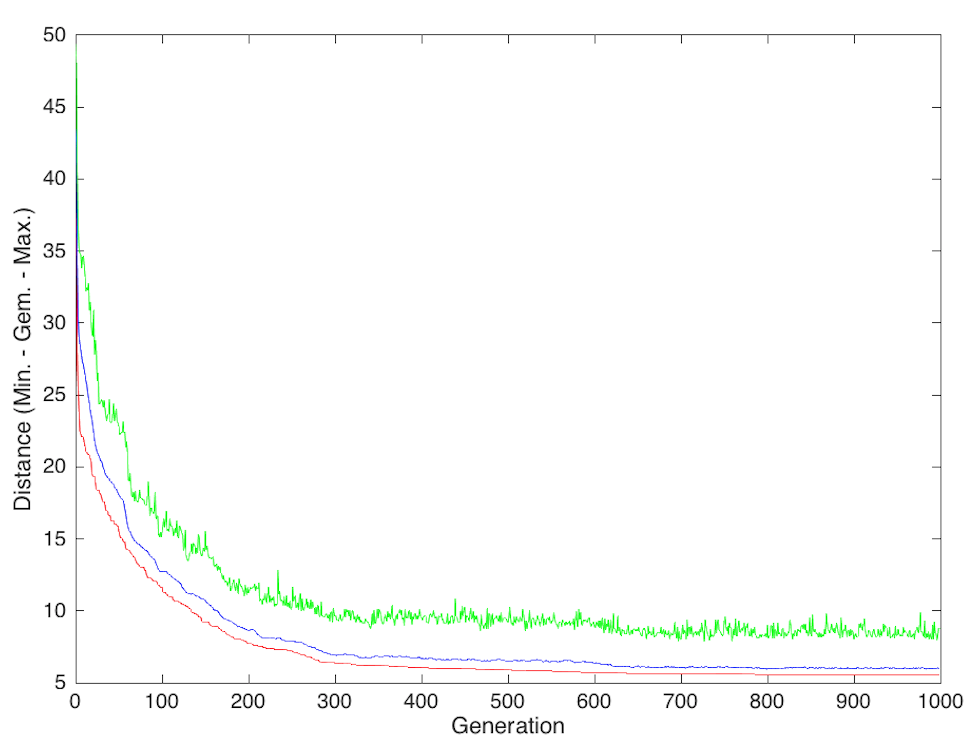
\includegraphics[width=0.7\textwidth]{../figures/figures_question_4/benchmark_131_gen}
      \caption{The fitness values (tour distances) for the best(red), average(blue) and worst(green) candidate solution in every generation. This figure corresponds to the problem solved in figure \ref{fig:benchmark_131_path}}
      \label{fig:benchmark_131_gen}
\end{figure}



\FloatBarrier